\documentclass[12pt]{article}
\linespread{1.2}
\usepackage[margin=2cm]{geometry}
\usepackage[utf8]{inputenc}
\usepackage{amsfonts}
\usepackage{amsmath}
\usepackage{multicol}
\usepackage{amsthm}
\usepackage{amssymb,scrextend}
\usepackage{graphicx,tikz}
\newtheorem{dfn}{Definition}
\renewcommand{\qed}{\hfill$\blacksquare$}
\let\newproof\proof
\renewenvironment{proof}{\vspace{1em}\begin{addmargin}[2em]{0em}\begin{newproof}}{\end{newproof}\end{addmargin}\qed}
\newenvironment{theorem}[2][Theorem]{\begin{trivlist}
\item[\hskip \labelsep {\bfseries #1} \hskip \labelsep {\bfseries #2.}]}{\end{trivlist}}
\newenvironment{example}[2][Example]{\begin{trivlist}
\item[\hskip \labelsep {\bfseries #1} \hskip \labelsep {\bfseries #2.}]}{\end{trivlist}}
\newenvironment{lemma}[2][Lemma]{\begin{trivlist}
\item[\hskip \labelsep {\bfseries #1} \hskip \labelsep {\bfseries #2.}]}{\end{trivlist}}
\newenvironment{exercise}[2][Exercise]{\begin{trivlist}
\item[\hskip \labelsep {\bfseries #1} \hskip \labelsep {\bfseries #2.}]}{\end{trivlist}}
\newenvironment{problem}[2][Problem]{\begin{trivlist}
\item[\hskip \labelsep {\bfseries #1} \hskip \labelsep {\bfseries #2.}]}{\end{trivlist}}
\newenvironment{corollary}[2][Corollary]{\begin{trivlist}
\item[\hskip \labelsep {\bfseries #1} \hskip \labelsep {\bfseries #2.}]}{\end{trivlist}}
\usepackage{fancyhdr,enumitem,changepage,url,tcolorbox}
\pagestyle{fancy}
\author{Warren Atkison}
\date{\today}
\setlength{\headheight}{15pt}
\begin{document}
\fancyhf{}
\fancyhead[L]{Warren Atkison}
\fancyhead[C]{Exam 2}
\fancyhead[R]{\today}
\fancyfoot[R]{\thepage}

\begin{tcolorbox}[colback = blue!5!white,colframe = blue!75!black]
	\begin{problem}{1}
		Show that all orbits of $F(z) = \lambda z$ are cycles if $\lambda = e^{2\pi i\frac{p}{q}}$, where $p,~q$ are integers.
	\end{problem}
\end{tcolorbox}
\begin{proof}
	Let $z_0 = re^{i\theta}$, then
	\begin{align*}
		z_1 &= re^{i\theta + 2\pi i \frac{p}{q}} \\
		z_2 &= re^{i\theta + 2\pi i \frac{2p}{q}} \\
		    &\vdots \\
		z_n &= re^{i\theta + 2\pi i \frac{np}{q}}
	\end{align*}
	At some point, $n = q$ and we have
	\[
		z_q = re^{i\theta + 2\pi i p} = re^{i\theta} = z_0
	\]
	since $p$ and $q$ are integers. Thus, all orbits of $F(z)$ are cycles.
\end{proof}
\begin{tcolorbox}[colback = blue!5!white,colframe = blue!75!black]
	\begin{problem}{2}
		Using Octave or Matlab, reproduce the figure at the top of page 139. For specificity, use $c = -1 - 2i$.
	\end{problem}
\end{tcolorbox}
	
\begin{figure}[h]
	\begin{center}
	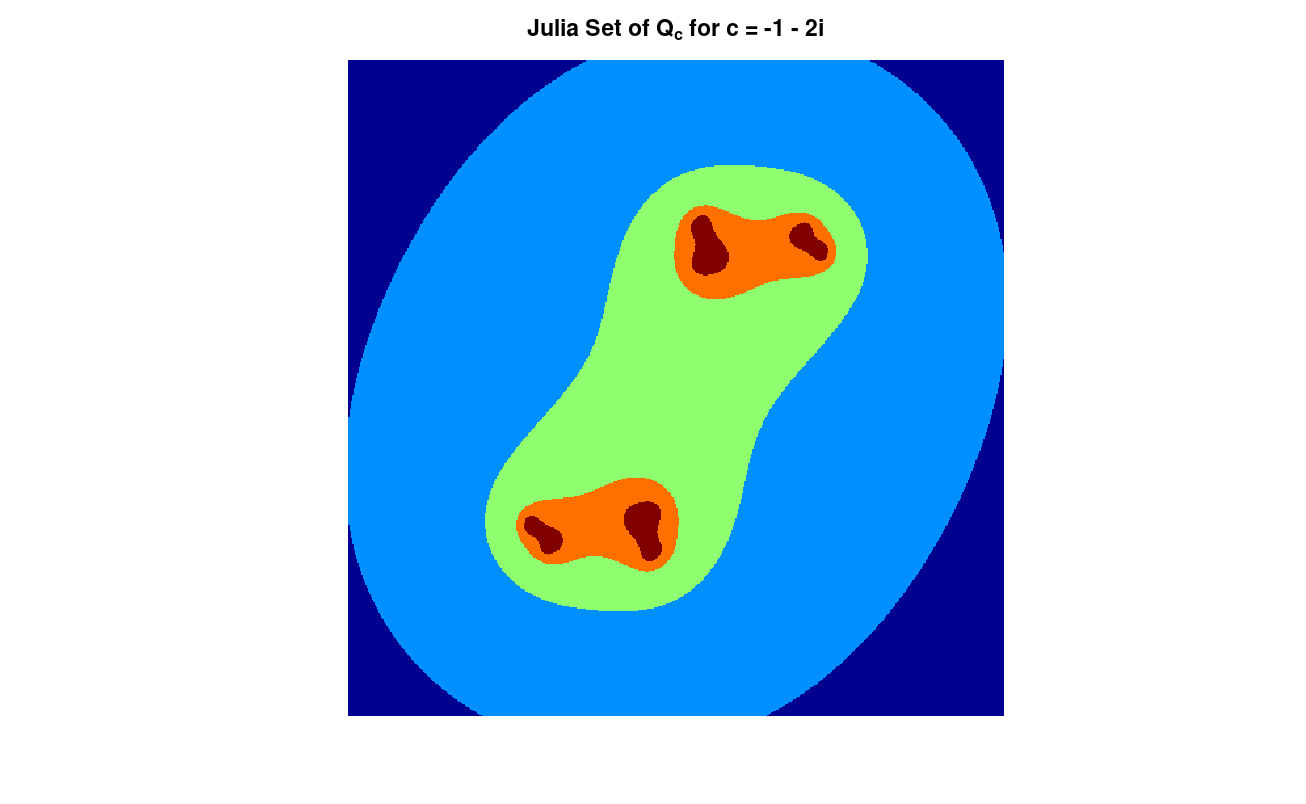
\includegraphics[scale = .3]{FigEX2.2.png}
	\caption{Filled Julia set for $c = -1-2i$}
	\end{center}
\end{figure}
\begin{tcolorbox}[colback=blue!5!white,colframe=blue!75!black]
	\begin{problem}{3a}
		Let $f: \mathbb{R} \to \mathbb{R}$ be continuous. Which of the following prime periods is possible without the other three and why?
		\[
			72,~114,~168,~172
		\]
	\end{problem}
\end{tcolorbox}

First we can do a prime decomposition of the four numbers.
\begin{align*}
	72 &= 2^3\cdot3^2 & 114 &= 2\cdot3\cdot19 & 168 &= 2\cdot3\cdot7 & 172 &= 2^2\cdot43
\end{align*}
	
Now we can apply Sharkovsky's Theorem which is as follows:
\begin{tcolorbox}[colback=red!5!white,colframe=red!75!black]
	\textbf{Sharkovsky's Theorem.} Suppose $F: \mathbb{R} \to \mathbb{R}$ is continuous. Suppose $F$ has a periodic point of prime period $n$ and that $n$ preceeds $k$ in the Sharkovsky ordering. Then $F$ also has a periodic point of prime period $k$.
\end{tcolorbox}
and the Sharkovsky ordering is
\begin{center}
	
\begin{tabular}{cccc}
	3 & 5 & 7 & \ldots \\
	$2\cdot3$ & $2\cdot5$ & $2\cdot 7$ & \ldots\\
	$2^2\cdot3$ & $2^2 \cdot 5$ & $2^2\cdot7$ & \ldots\\
		    & \vdots && \\
	\ldots & $2^n$ & \ldots & $2^0$
\end{tabular}

\end{center}

The prime which appears last in the Sharkovsky ordering doesn;t imply the rest, so 72 is the possilbe prime period which is possilbe without the rest.

\begin{tcolorbox}[colback=blue!5!white,colframe=blue!75!black]
	\begin{problem}{3b}
		Show that if $F(x_1) < a$ and $F(x_2) > a$ then Period 4 implies Period 2.
	\end{problem}	
\end{tcolorbox}
\begin{proof}
	First we have that $F(x_1) = x_2$. Let $I_0 = [x_3,x_4]$ and $I_1 = [x_2,x_3]$. Then we have that $F(I_0) \supset I_1$ and $F(I_1) \supset I_0 \cup I_1 $ since. From here he have the same situation with Period 3 points, so we have a Period 2 cycle
\end{proof}
\begin{tcolorbox}[colback=blue!5!white,colframe=blue!75!black]
	\begin{problem}{4a}
		Compute the Schwarzian derivative of a polynomial $P$ if $P'(x) = -2(x+1)(x-2)(x-3)$, by computing the derivative of $\ln|P'(x)|$.
	\end{problem}
\end{tcolorbox}

First we have
\begin{align*}
	\ln(P'(x)) = \ln(-2(x+1)(x-2)(x-3)) = \ln(-2) + \ln(x+1) + \ln(x-2) + \ln(x-3)
\end{align*}

We can take the derivative using the chain rule to get
\begin{align*}
	\frac{P''(x)}{P'(x)} = \frac{1}{x + 1} + \frac{1}{x - 2} + \frac{1}{x - 3}
\end{align*}

Differentiating again we find
\begin{align*}
	\frac{P'''(x)P'(x) - (P''(x))^2}{(P'(x))^2} &= \frac{P'''(x)}{P'(x)} - \left(\frac{P''(x)}{P'(x)}\right)^2 \\
						    &= -\frac{1}{(x+1)^2} - \frac{1}{(x-2)^2} - \frac{1}{(x-3)^2}
\end{align*}

Now we can compute the Schwarzian.
\begin{align*}
	SP(x) &= \frac{P'''(x)}{P'(x)} - \left(\frac{P''(x)}{P'(x)}\right)^2 - \frac{1}{2}\left(\frac{P''(x)}{P'(x)}\right) \\
	      &= -\frac{1}{(x+1)^2} - \frac{1}{(x-2)^2} - \frac{1}{(x-3)^2} - \frac{1}{2}\left(\frac{1}{x + 1} + \frac{1}{x - 2} + \frac{1}{x - 3}\right)^2
\end{align*}

\begin{tcolorbox}[colback=blue!5!white,colframe=blue!75!black]
	\begin{problem}{4b}
		In a short essay, summerize the importance of the Schwarzian derivative in our construction of the Mandlebrot set.
	\end{problem}	
\end{tcolorbox}

The Schwarzian derivative has many principles that make the can simplify the analysis of dynamic systems. One important principle is the Schwarzian min-max Principle: if $SF < 0$, then $F'$ cannot have a positive local minimum or a negative local maximum, so if a function has a negative Schwarzian derivative then it can only have a certain shape. Another property that follows from this the following: If $SF < 0$ and $x_0$ is an attracting periodic point of $F$, then either the imediate basin of attraction of $x_0$ extends to $+\infty$ or $-\infty$, or else there is a critical point of $F$ whose orbit is attracted to $x_0$.

This property can be used to analyze the local dynamics around critical points for any given $c$ of the Mandlebrot set. We can classify critical points as either stable or neutral with this theorem which can help determine regions belonging to the Mandlebrot set without much computation.
\begin{tcolorbox}[colback=blue!5!white,colframe=blue!75!black]
	\begin{problem}{5}
		Let $F(x) = x/(x-1)$. Find the fixed points for Newton's iteration function and determine if they are attracting or repelling. Does your conlusion match what you expect?
	\end{problem}	
\end{tcolorbox}

First we find the derivative of $F$.
\begin{align*}
	F'(x) = \frac{(x-1) - x}{(x-1)^2} = -\frac{1}{(x-1)^2}
\end{align*}

Then we compute Newton's iteration function for $F$.
\begin{align*}
	N(x) = x - \frac{F(x)}{F'(x)} = x - \dfrac{x/(x-1)}{-1/(x-1)^2} = x + x(x - 1)
\end{align*}

Now we can find the fixed points.
\begin{align*}
	x = x + x(x-1) \implies x(x-1) = 0
\end{align*}

so $x = 0$ and $x = 1$ are fixed points for $N(x)$. To determine if these points are attracting or repelling, we can find the derivative of $N(x)$.
\[
	N'(x) = 1 + 2x - 1 = 2x
\]
$|N'(0)| = 0$ so we have an attracting point at $x=0$, and $|N'(1)| = 2$ so we have a repelling point at $x = 1$. This makes sense becuase at $F(0) = 0$, so we'd want that to be an attracting fixed point, and at $x = 1$ $F$ goes to infinity, so we'd want that to be a repelling fixed point.
\begin{tcolorbox}[colback=blue!5!white,colframe=blue!75!black]
	\begin{problem}{6}
		Consider $Q_c(z) = z^2 + i$.
		\begin{itemize}
			\item[(a)] Show that the orbit of 0 is eventaully periodic.
			\item[(b)] Show that the periodic orbit you found is either attracting or repelling
			\item[(c)] Use the random iteration algorithm to produce a sketch of the Julia set. Should it be connected or disconnected?
		\end{itemize}
	\end{problem}	
\end{tcolorbox}
\begin{itemize}
	\item[(a)] When $z = 0$, the orbit of $Q_i$ is as follows.
		\begin{align*}
			0 \to i \to -1 + i \to -2i + i = -i \to -1 + i
		\end{align*}

		As we can see the orbit of 0 is eventaully periodic to the Period 2 cycle of $z_0 = -1 + i$ or $z_0 = -i$.
	\item[(b)] Since we know the period 2 cycle we want, we can find $|(Q_c^2)'(-i)|$ as follows.
		\begin{align*}
			|(Q_c^2)'(-i)| &= |Q_c'(-i) \cdot Q_c'(-1 + i)| \\
				     &= |2(-i)\cdot2(-1 + i)| \\
				     &= |4(i + 1)| \\
				     &> 1
		\end{align*}
		so this cycle is repelling.
	\item[(c)] Here is the Julia set of $Q_i$.
		\begin{figure}[ht]
			\begin{center}
				
			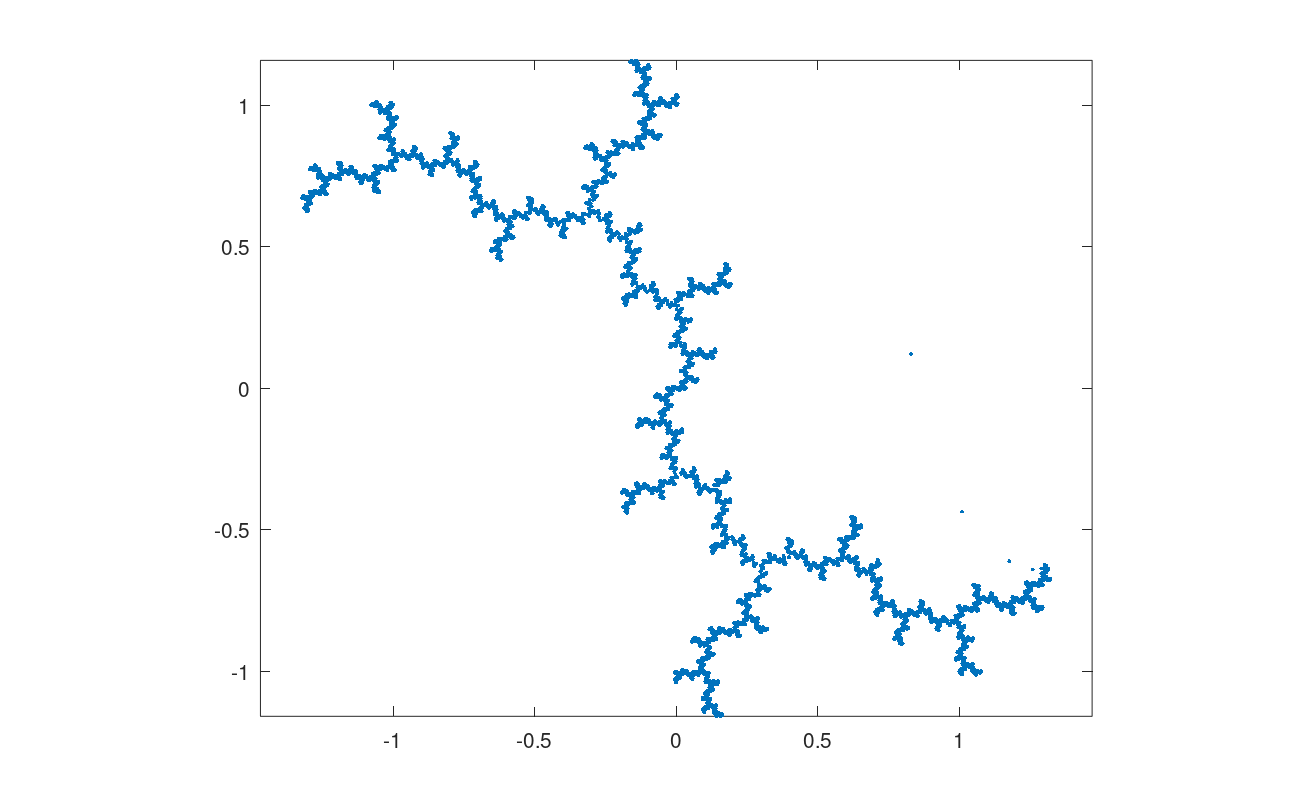
\includegraphics[scale=.35]{FigEX2.6c.png}
			\caption{Julia set of $c = i$ using random iteration}
			\end{center}
		\end{figure}
		Since we had an eventaully repelling fixed point at $z = 0$ which is a critical point, it makes sense that the Julia set would be disconnected, or a dusting of points
\end{itemize}
\end{document}
